%%%%%%%%%%%%%%%%%%%%%%%%%%%%%%%%%%%%%%%%%
% a0poster Portrait Poster
% LaTeX Template
% Version 1.0 (22/06/13)
%
% The a0poster class was created by:
% Gerlinde Kettl and Matthias Weiser (tex@kettl.de)
% 
% This template has been downloaded from:
% http://www.LaTeXTemplates.com
%
% License:
% CC BY-NC-SA 3.0 (http://creativecommons.org/licenses/by-nc-sa/3.0/)
%
%%%%%%%%%%%%%%%%%%%%%%%%%%%%%%%%%%%%%%%%%

%----------------------------------------------------------------------------------------
%	PACKAGES AND OTHER DOCUMENT CONFIGURATIONS
%----------------------------------------------------------------------------------------

\documentclass[a0,portrait]{a0poster}

\usepackage{multicol} % This is so we can have multiple columns of text side-by-side
\columnsep=100pt % This is the amount of white space between the columns in the poster
\columnseprule=3pt % This is the thickness of the black line between the columns in the poster

\usepackage[svgnames]{xcolor} % Specify colors by their 'svgnames', for a full list of all colors available see here: http://www.latextemplates.com/svgnames-colors

\usepackage{times} % Use the times font
%\usepackage{palatino} % Uncomment to use the Palatino font

\usepackage{graphicx} % Required for including images
\graphicspath{{figures/}} % Location of the graphics files
\usepackage{booktabs} % Top and bottom rules for table
\usepackage[font=small,labelfont=bf]{caption} % Required for specifying captions to tables and figures
\usepackage{amsfonts, amsmath, amsthm, amssymb} % For math fonts, symbols and environments
\usepackage{wrapfig} % Allows wrapping text around tables and figures
\newcommand{\mat}[1]{\bm{#1}}
\newcommand{\tens}[1]{\bm{\mathcal{#1}}}
\newcommand{\tensel}[1]{\mathcal{#1}}
\newcommand{\GP}{\mathcal{GP}}
\newcommand{\E}{\mathbb{E}}
\newcommand{\R}{\mathbb{R}}
\newcommand{\N}{\mathcal{N}}
\newcommand{\bigO}{\mathcal{O}}
\newcommand{\cov}{\mbox{cov}}
\newcommand{\KL}[2]{\mbox{KL}\left(#1\mbox{ || }#2\right)}
\newcommand{\tr}{\mbox{tr}}

\begin{document}

%----------------------------------------------------------------------------------------
%	POSTER HEADER 
%----------------------------------------------------------------------------------------

% The header is divided into two boxes:
% The first is 75% wide and houses the title, subtitle, names, university/organization and contact information
% The second is 25% wide and houses a logo for your university/organization or a photo of you
% The widths of these boxes can be easily edited to accommodate your content as you see fit

\begin{minipage}[b]{1.\linewidth}
  \begin{center}
  \veryHuge \color{NavyBlue} 
    \textbf{Scalable Gaussian Processes with Billions of Inducing Inputs \\via Tensor Train Decomposition} \color{Black}\\ % Title
\huge \textbf{Pavel Izmailov\textsuperscript{1,4} \quad Alexander Novikov\textsuperscript{2,3} \quad Dmitry Kropotov\textsuperscript{4}}\\[0.5cm] % Author(s)
\huge \textsuperscript{1} Cornell University 
  \quad 
  \textsuperscript{2} National Research University Higher School of Economics\\
  \quad 
  \textsuperscript{3} Institute of Numerical Mathematics RAS
  \quad 
  \textsuperscript{4} Lomonosov Moscow State University
  \\[0.4cm] % University/organization
\end{center}
\Large \texttt{izmailovpavel@gmail.com} %--- 1 (000) 111 1111\\
\end{minipage}
%
%\begin{minipage}[b]{0.25\linewidth}
%\includegraphics[width=20cm]{logo.png}\\
%\end{minipage}

\vspace{1cm} % A bit of extra whitespace between the header and poster content

%----------------------------------------------------------------------------------------

\begin{multicols}{2} % This is how many columns your poster will be broken into, a portrait poster is generally split into 2 columns

%----------------------------------------------------------------------------------------
%	ABSTRACT
%----------------------------------------------------------------------------------------

%\begin{abstract}
%
%Abstract
%\end{abstract}

\section*{\LARGE \color{NavyBlue}Motivation}

Motivation

\section*{\LARGE \color{NavyBlue} Tensor Train Format}


\begin{center}
    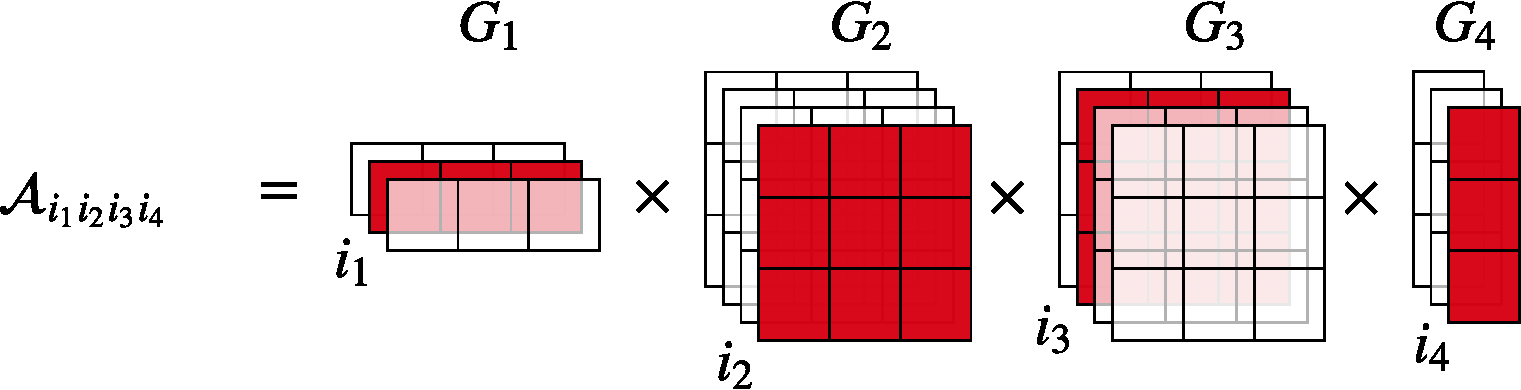
\includegraphics{pics/tt/TT_v2.pdf}
\end{center}
Intro

\section*{\LARGE \color{NavyBlue}Gaussian Process ELBO}

\section*{\LARGE \color{NavyBlue}TT-GP}

\section*{\LARGE \color{NavyBlue} Properties}

\section*{\LARGE \color{NavyBlue} Experiments}
\subsection*{\large \color{NavyBlue} RBF kernel}
\subsection*{\large \color{NavyBlue} Deep kernels}



\nocite{*} % Print all references regardless of whether they were cited in the poster or not
\bibliographystyle{plain} % Plain referencing style
\bibliography{sample} % Use the example bibliography file sample.bib

%\section*{Acknowledgements}


\end{multicols}
\end{document}
